\documentclass{beamer}
\usetheme{Boadilla}

\usepackage[utf8]{inputenc}
%tohle nejak nefunguje, ale ceske znaky se kresli i bez toho\usepackage[czech]{babel}

\title{Generování matic bez zakázaných vzorů}
\author{Stanislav Kučera}
\institute[IÚUK]{Informatický ústav Univerzity Karlovy}
\date{8.~9.~2016}

\begin{document}

\begin{frame}
\titlepage
% Dobrý den, jmenuji se Stanislav Kučera a vítám vás na své obhajobě.
% Jako svou bakalářskou práci jsem se svým vedoucím, Vítem Jelínkem navrhl a implementoval několik algoritmů, které dohromady tvoří program generující matice bez zakázaných vzorů.
\end{frame}

\begin{frame}
\frametitle{Obsah}
\tableofcontents
% Nejprve by asi stálo za zmínku, co to jsou matice bez zakázaných vzorů a proč vlastně chceme takové matice generovat.
% Potom si ukážeme některé algoritmy a jejich vylepšení, které jsou v mé práci obsaženy.
\end{frame}

\section{Zakázané vzory}
\subsection{Definice}
\begin{frame}
\frametitle{Zakázaný vzor}
\begin{block}{Definice}
Binární matice $M\in\{0,1\}^{m\times n}$ \emph{obsahuje} binární matici $P\in\{0,1\}^{k\times l}$ \emph{jako podmatici}, pokud lze z~$M$ vynecháním některých řádků a~sloupečků získat matici $M'$ $k\times l$ takovou, že pokud má $P$ jedničku na~nějaké pozici, má na~téže pozici jedničku i~$M'$. Jinak řekneme, že $M$ \emph{neobsahuje (vyhýbá se)} $P$ \emph{jako podmatici}.
%. Přečtu?
\end{block}
\vspace{5mm}
\centering
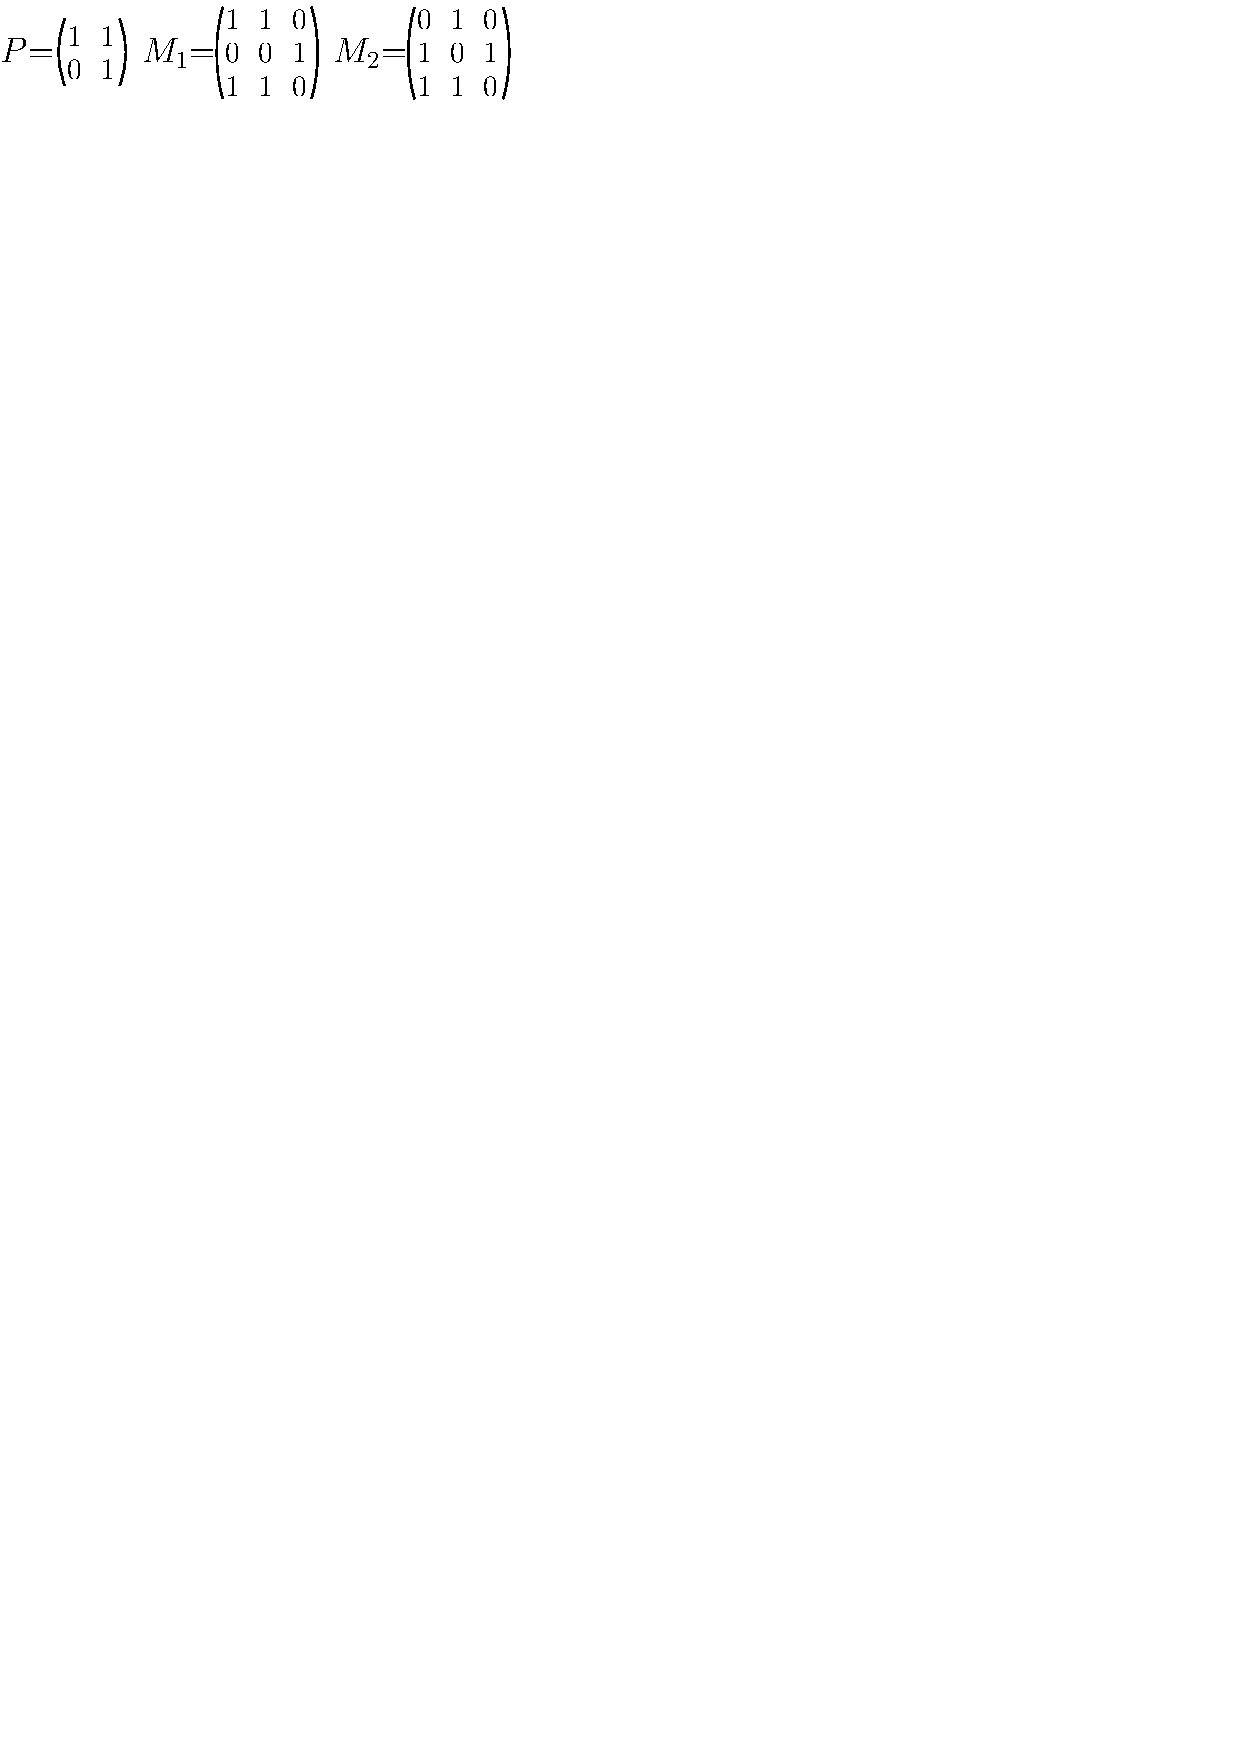
\includegraphics{../img/example.pdf}<1>
% Nejlépe je to vidět na obrázku, kde matice M_1 obsahuje P, protože vynecháním prostředního řádku a posledního sloupce dostaneme podmatici, která má jedničky tam, kde je má vzor. Naopak matice M_2 vzor P neobsahuje
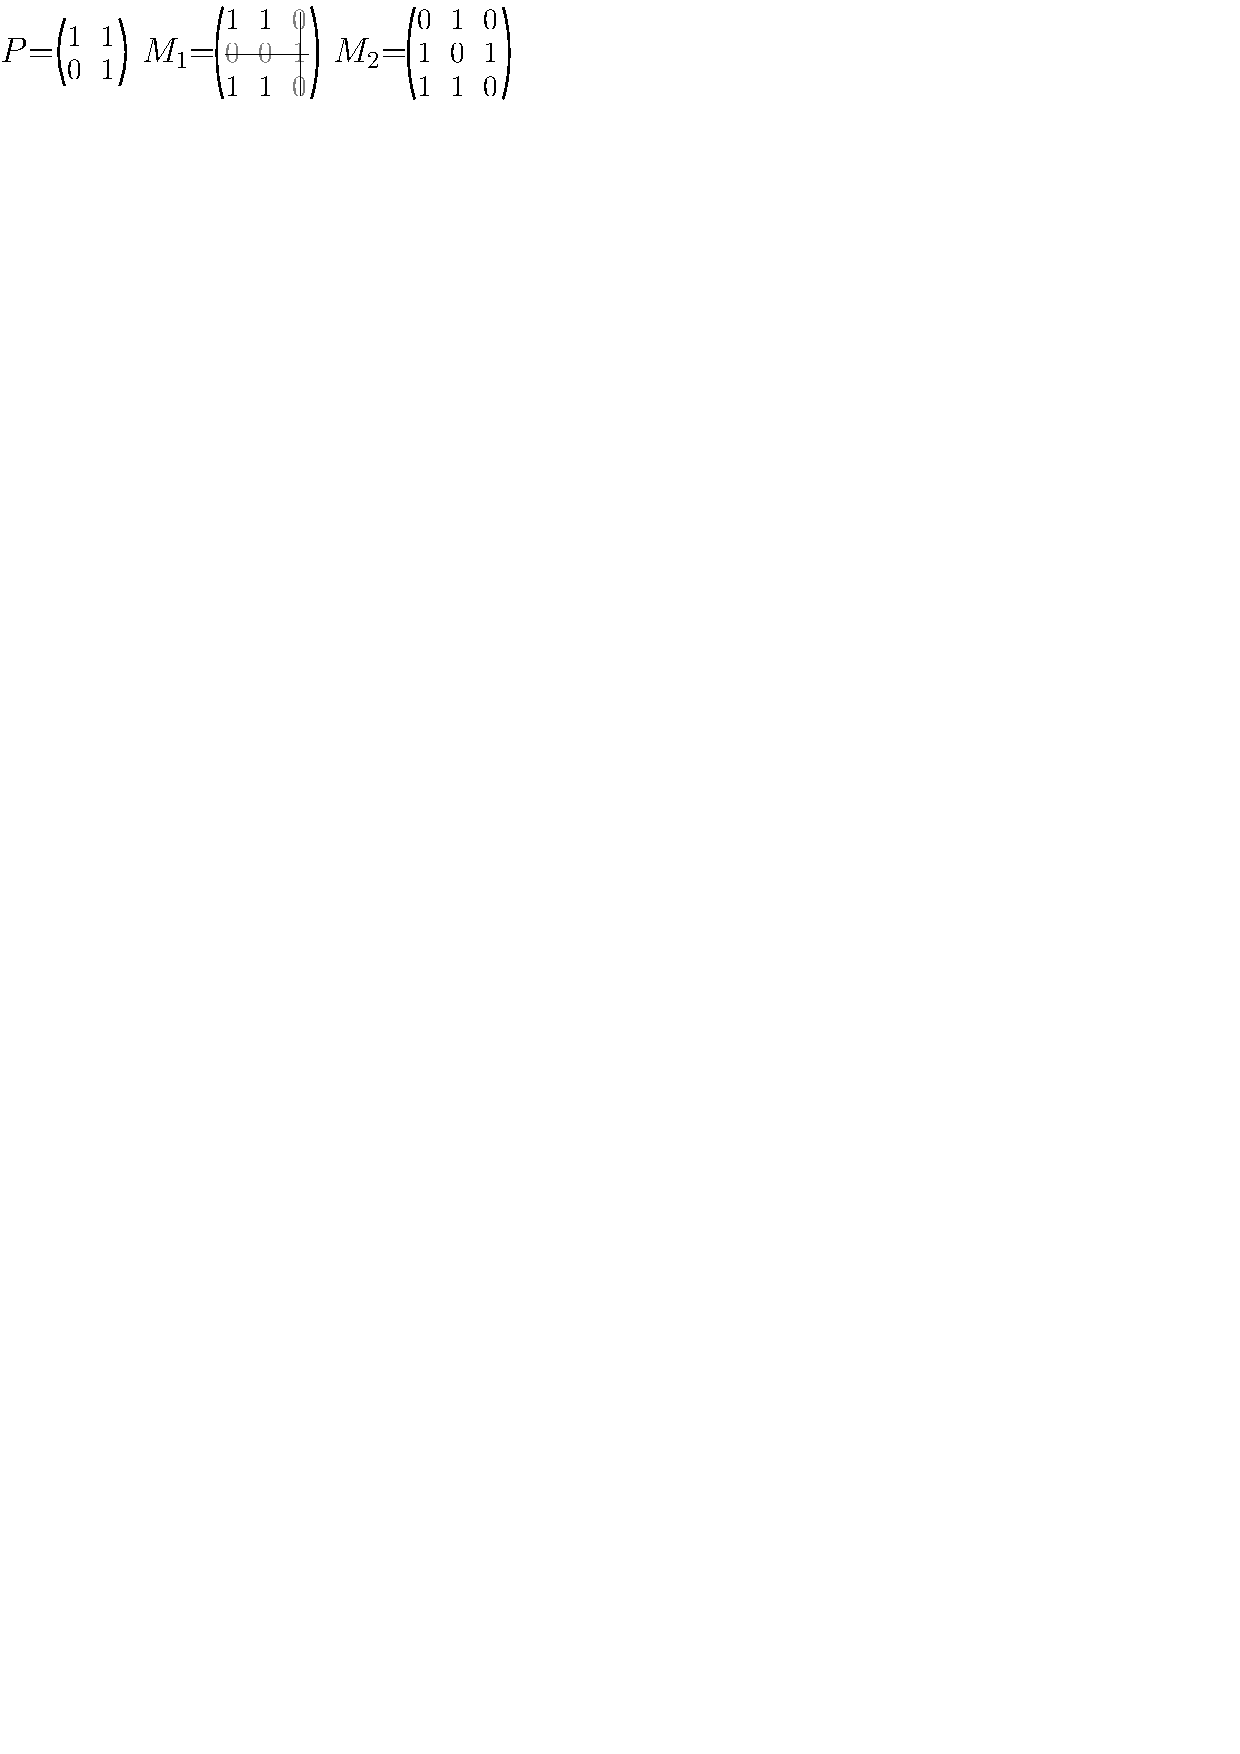
\includegraphics{../img/example2.pdf}<2>
\end{frame}

\subsection{Příklady použití}
\begin{frame}
\frametitle{Příklady použití}
\begin{itemize}
\setlength\itemsep{3mm}
\item Pomocí matic bez~zakázaných vzorů se~dokázal horní odhad časové složitosti algoritmu Efrata a~Sharira na~``Segment-center problem''.
%?za český překlad budu vděčný, podobný problém ``$k$ center problem'' se překládá jako ``problém $k$ center'', můj nejlepší překlad je ``problém centrování úsečky'', ale nikde jsem to nenašel a ani někomu, kdo ten problém zná ten český název možná nic neřekne.
\item Existuje korelace mezi některými třídami matic bez~zakázených vzorů a~Davenport-Schinzelovým posloupnostmi, které zase korelují se~složitostí dolní (horní) obálky arrangementů v~rovině.
%. Nejspíš jen přečtu, případně vysvětlím, kdyby se někdo zeptal.
% Teď, když vidíme, že může být zajímavé zkoumat třídy matic, které neobsahují zakázaný vzor, co může být pro testování hypotéz užitečnější, než si umět vygenerovat matici z libovolné třídy, která je náhodná.
%? Měl bych tohle citovat? Oba zdroje mám, ale nevám, zda je to nutné.
\end{itemize}
\end{frame}

% Přidat slide s ukázkou vygenerované matice bez walking_pattern?

\section{Generování matic}
\subsection{Teoretické pozadí}
\begin{frame}
\frametitle{Markovovy řetězce}
\begin{block}{Definice (neformální)}
Pro předepsané pravděpodobnosti $p_{i,j}$ je \emph{Markovův řetězec} posloupnost prvků $X_0,\dots$ ze~stavové množiny $\mathcal{X}$ dodržující $P[X_{t+1}=j|X_t=i]=p_{i,j}.$
\end{block}
%. Přečtu svými slovy.
\pause
\begin{block}{Věta (neformální)}
Pokud je Markovův řetězec aperiodický, nerozložitelný a~symetrický, potom je jeho limita uniformně náhodně rozložena na stavové množině $\mathcal{X}$.
\end{block}
%? Tady by se skoro hodilo citovat nebo napsat jméno autora, ale autora jsem nenašel a nevím, jestli zase citovat Madrase, který to své knize ani nedokazuje, nebo se pokusit jít někam hlouběji?
% Klíčová věta, na které stojí můj celý program.
%. Přečtu.
\end{frame}

\begin{frame}
\frametitle{Markovův řetězec pro matice}
Pokud chceme generovat matici neobsahující vzor $P$, postupujeme takto:
\begin{enumerate}
\item Zvolíme libovolnou matici $M$ neobahující $P$.
\item Změníme uniformně náhodně vybraný bit $M$, čímž dostaneme $M'$.
\item Pokud $M'$ neobsahuje $P$ jako podmatici, nastavíme $M:=M'$.
\item Goto 2.
\end{enumerate}
%. Přečtu svými slovy.
\vspace{1em}
\pause
Protože definovaný Markovův řetězec splňuje předpoklady věty z~minulého slidu, jeho limita je náhodná matice neobsahující vzor $P$ jako podmatici. My ale nemáme čas čekat nekonečně dlouho, a~zároveň zmíněná věta ani~žádná jiná nedává odhad na~dostačující počet iterací (mixing time), takže volbu počtu iterací necháme na~uživateli.
%. Přečtu.
\end{frame}

\subsection{Algoritmus pro testování speciálních vzorů}
\begin{frame}
\frametitle{Algoritmus pro testování speciálních vzorů}
\begin{block}{Definice}
O~matici řekneme, že je to Walking pattern, pokud existuje procházka z~levého horního rohu matice do~pravého dolního rohu obsahující všechny jedničky v~matici.
\end{block}
%? Procházkový vzor?
%. Přečtu a zmíním, že procházka je monotónní.
\vspace{5mm}
\centering
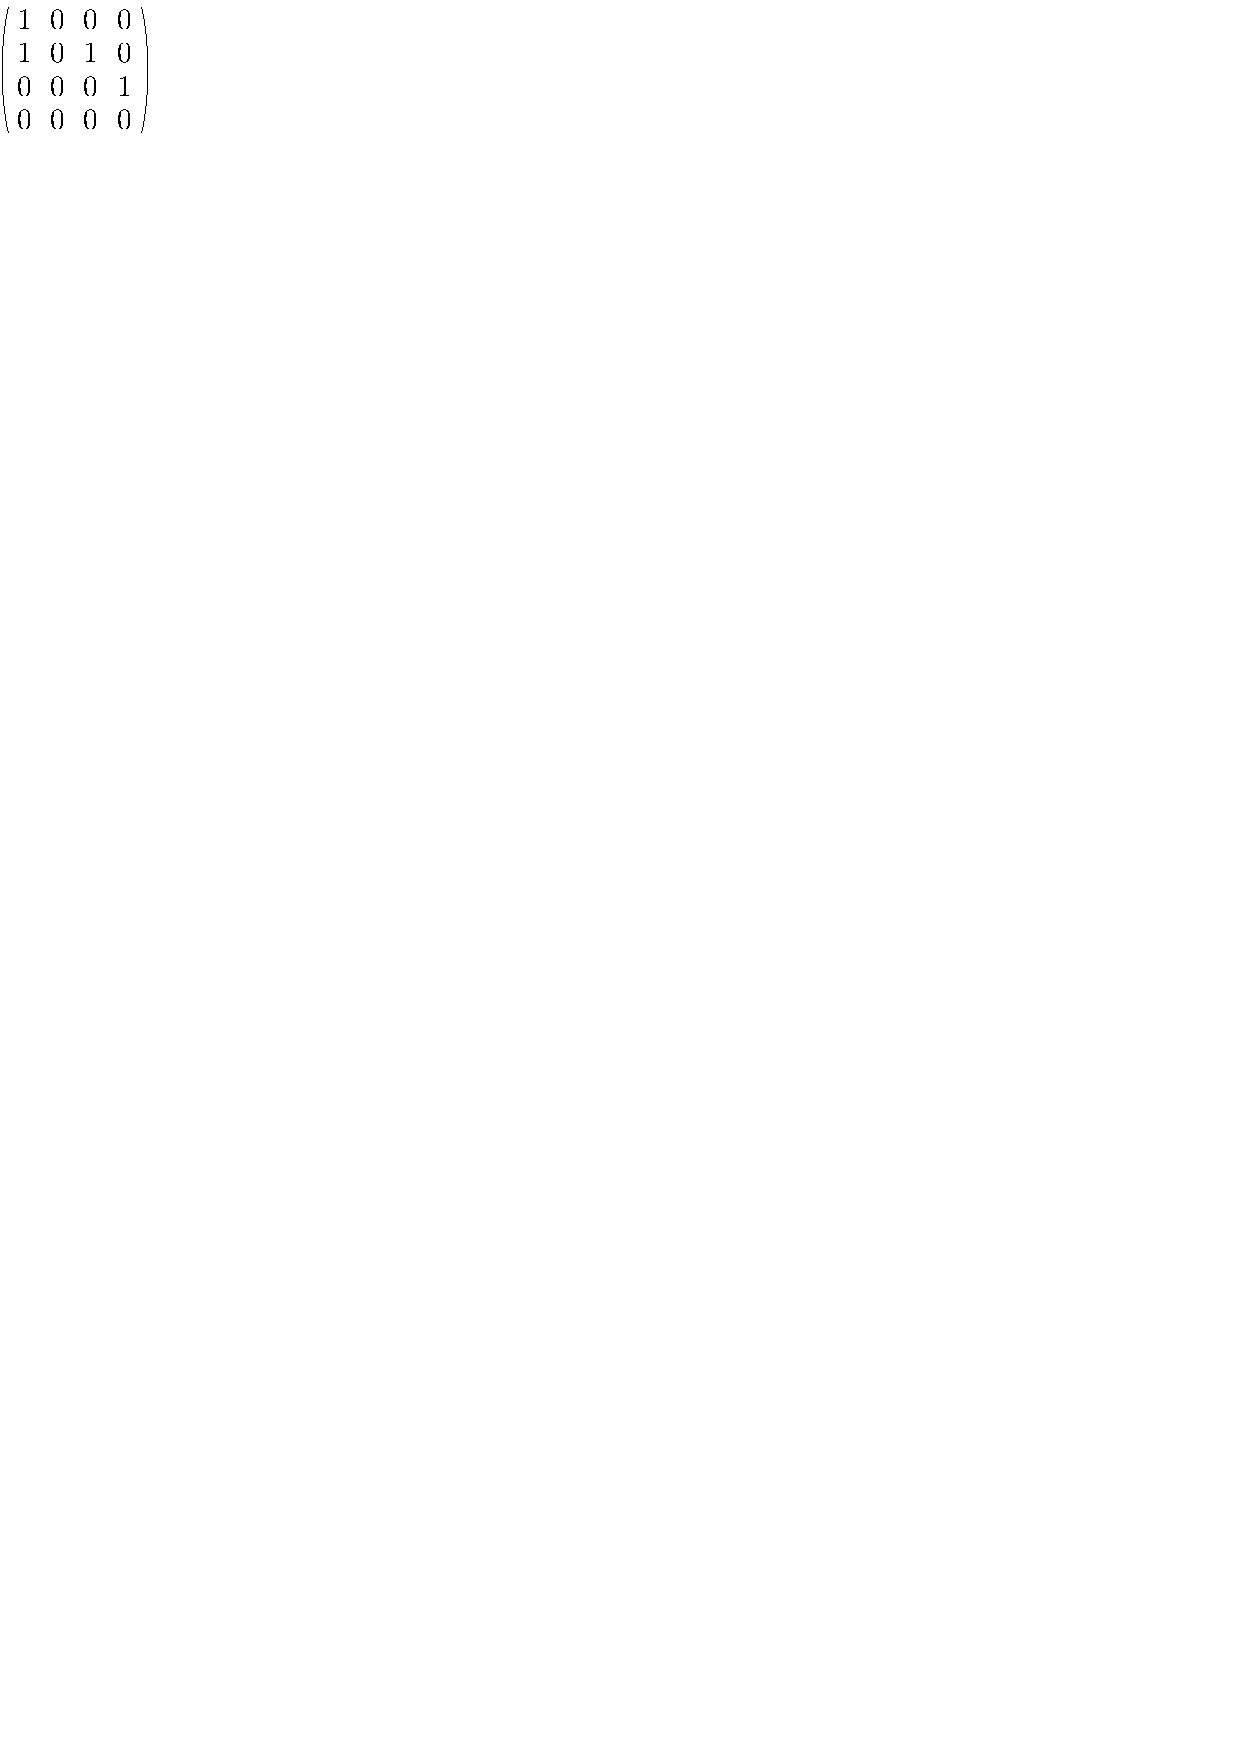
\includegraphics{../img/walkingexample1.pdf}<1>
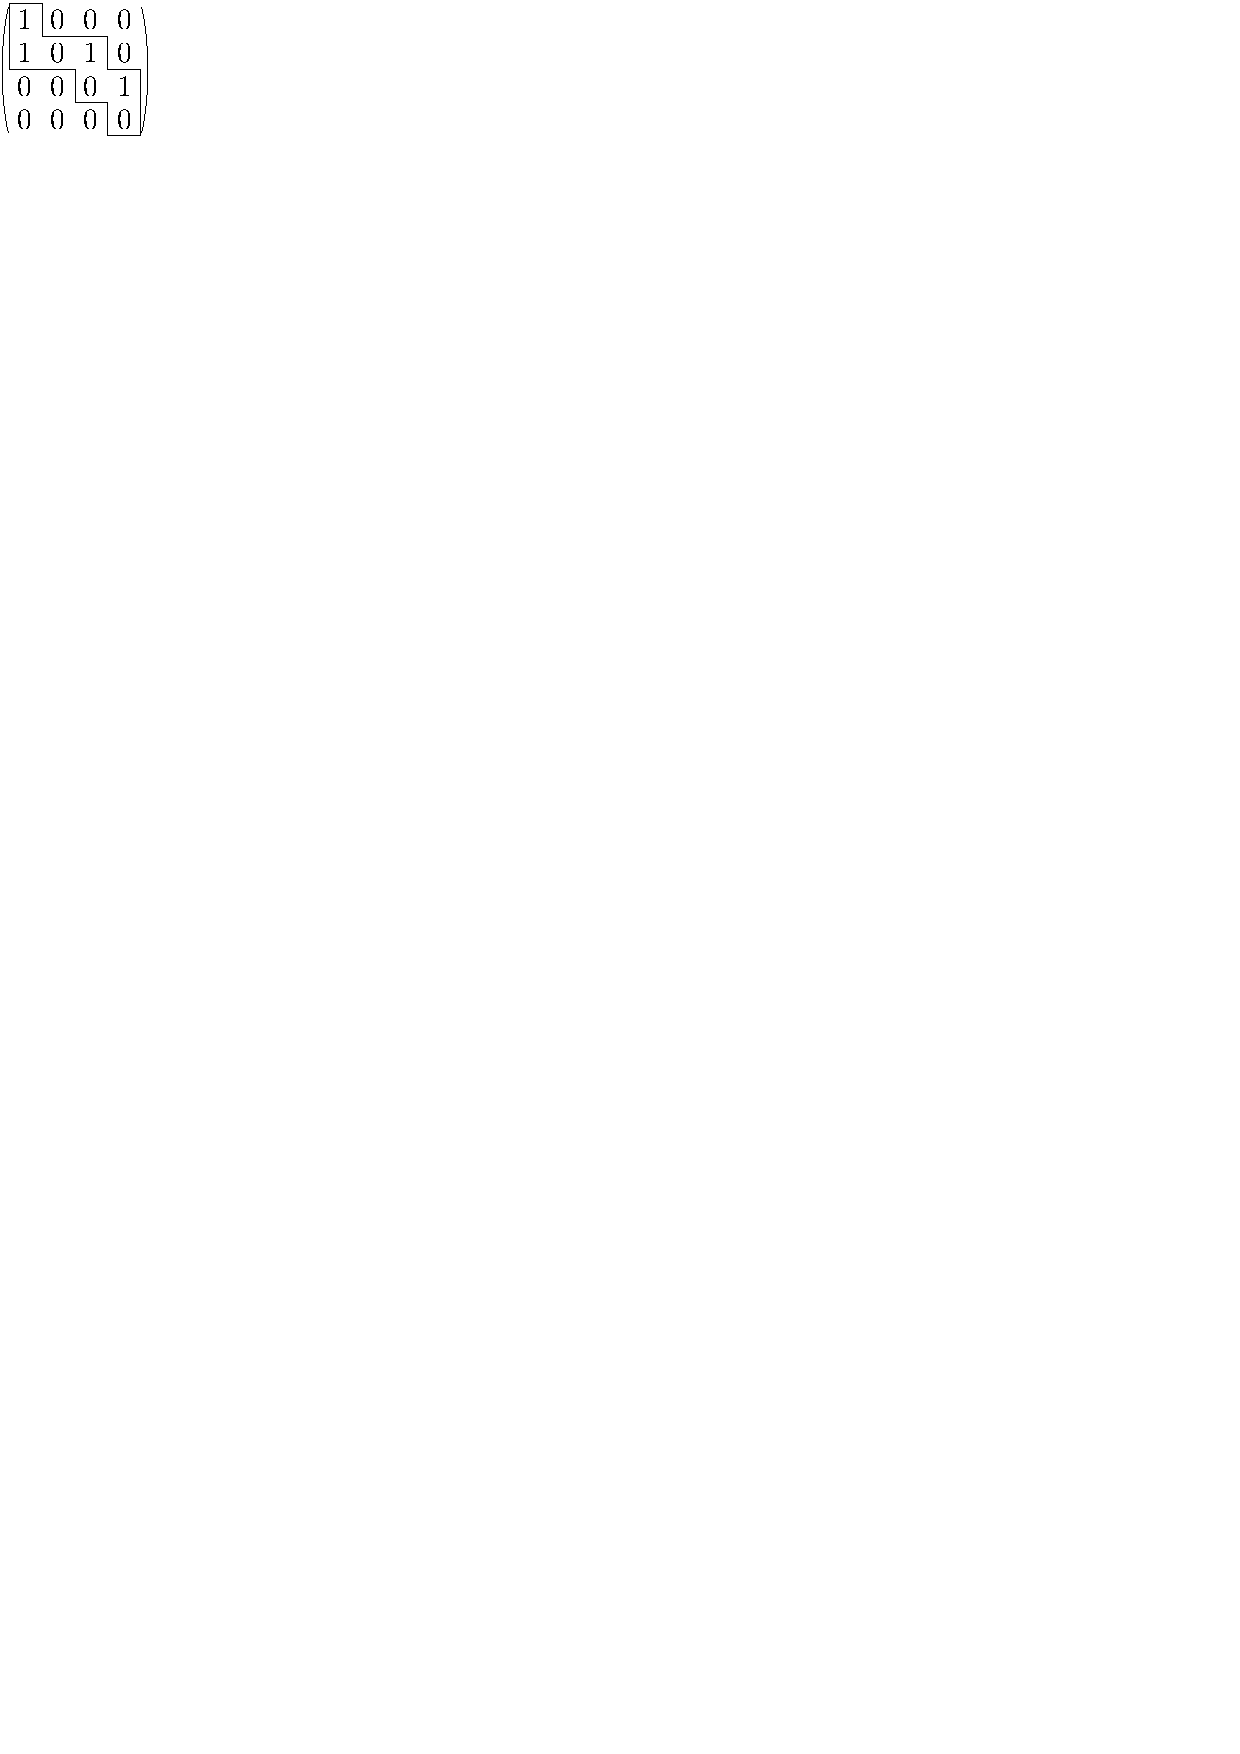
\includegraphics{../img/walkingexample2.pdf}<2>
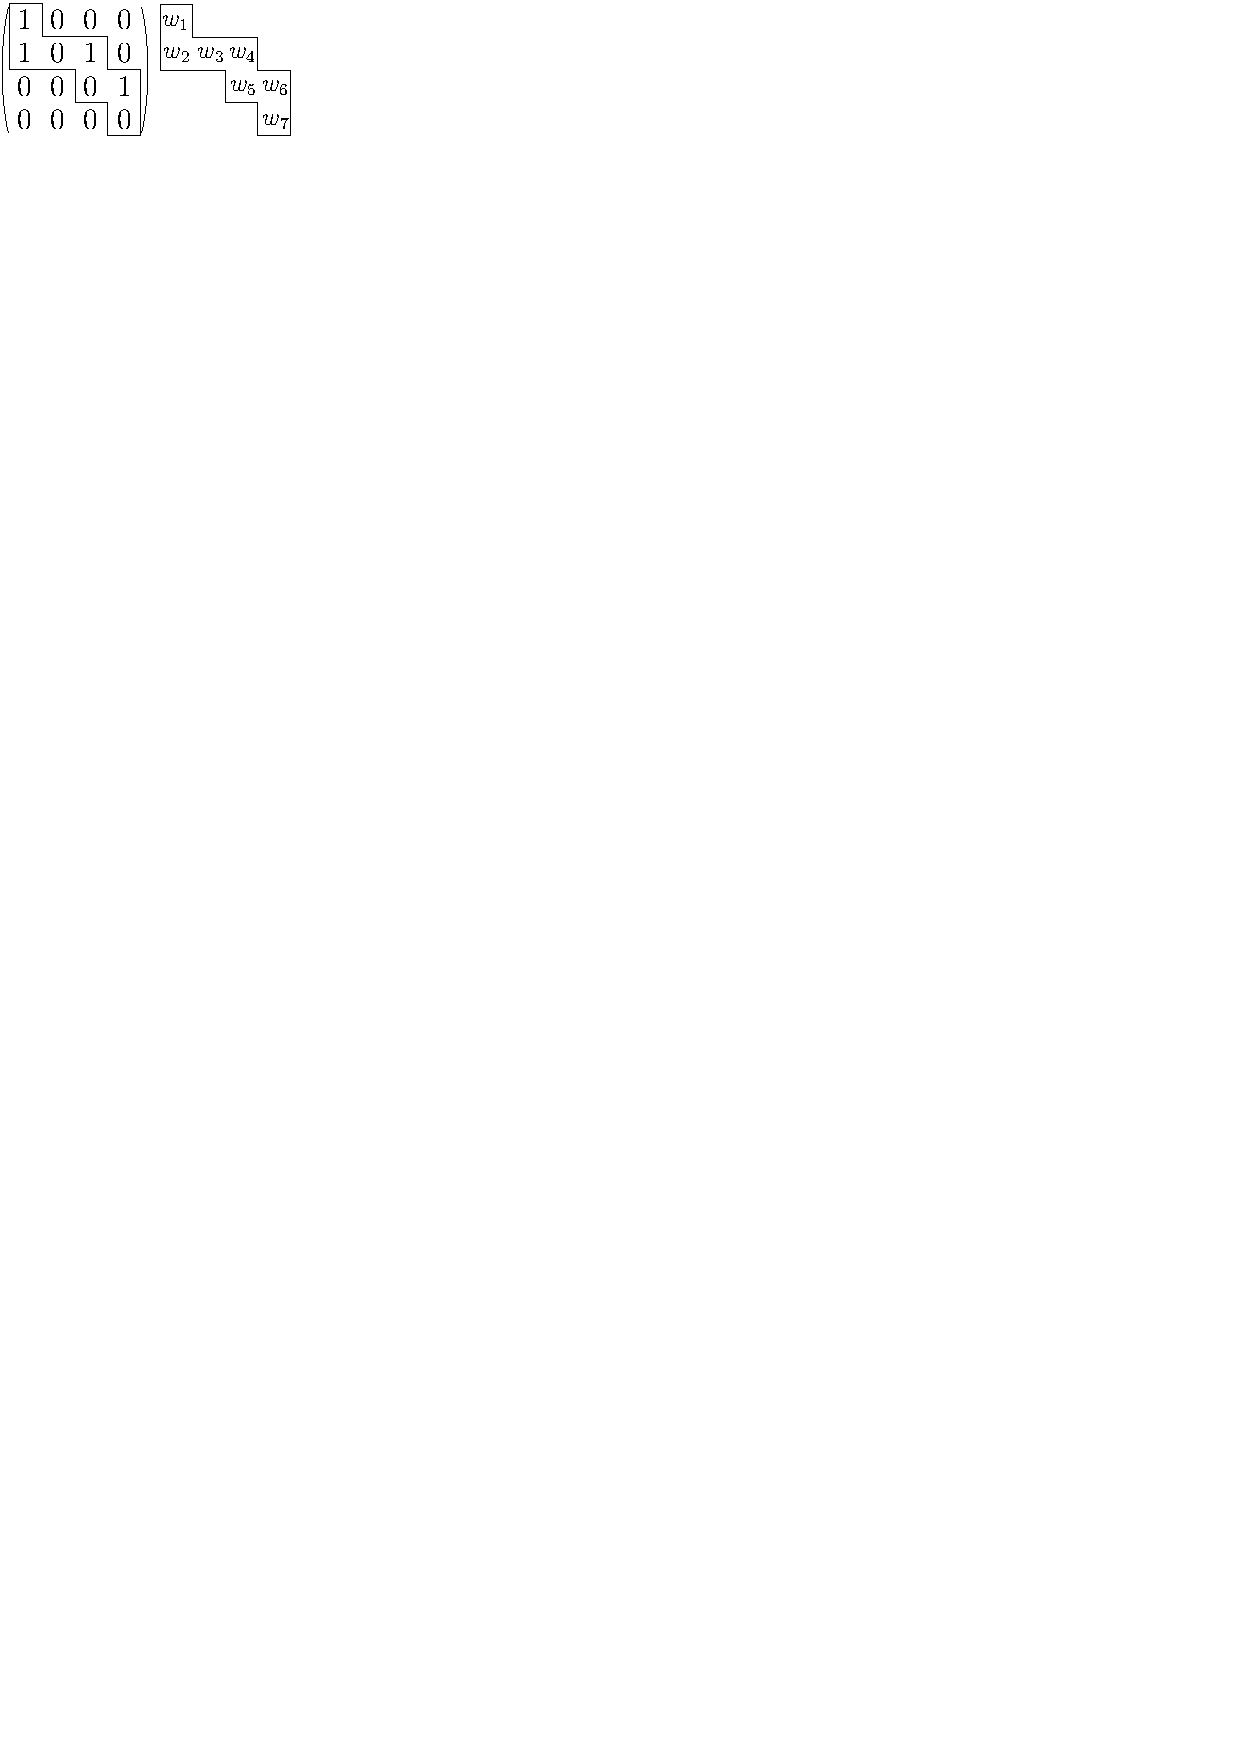
\includegraphics{../img/walkingexample3.pdf}<3>
% Na obrázku máme jeden takový vzor. Ona procházka je vyznačena v rámečku a všechny prvky procházky se ještě naznačeným způsobem oindexujeme.
\end{frame}

\begin{frame}
\frametitle{Algoritmus pro testování Walking pattern}
\centering

\includegraphics[scale=1.5]{../img/walkingalg0.pdf}<1>
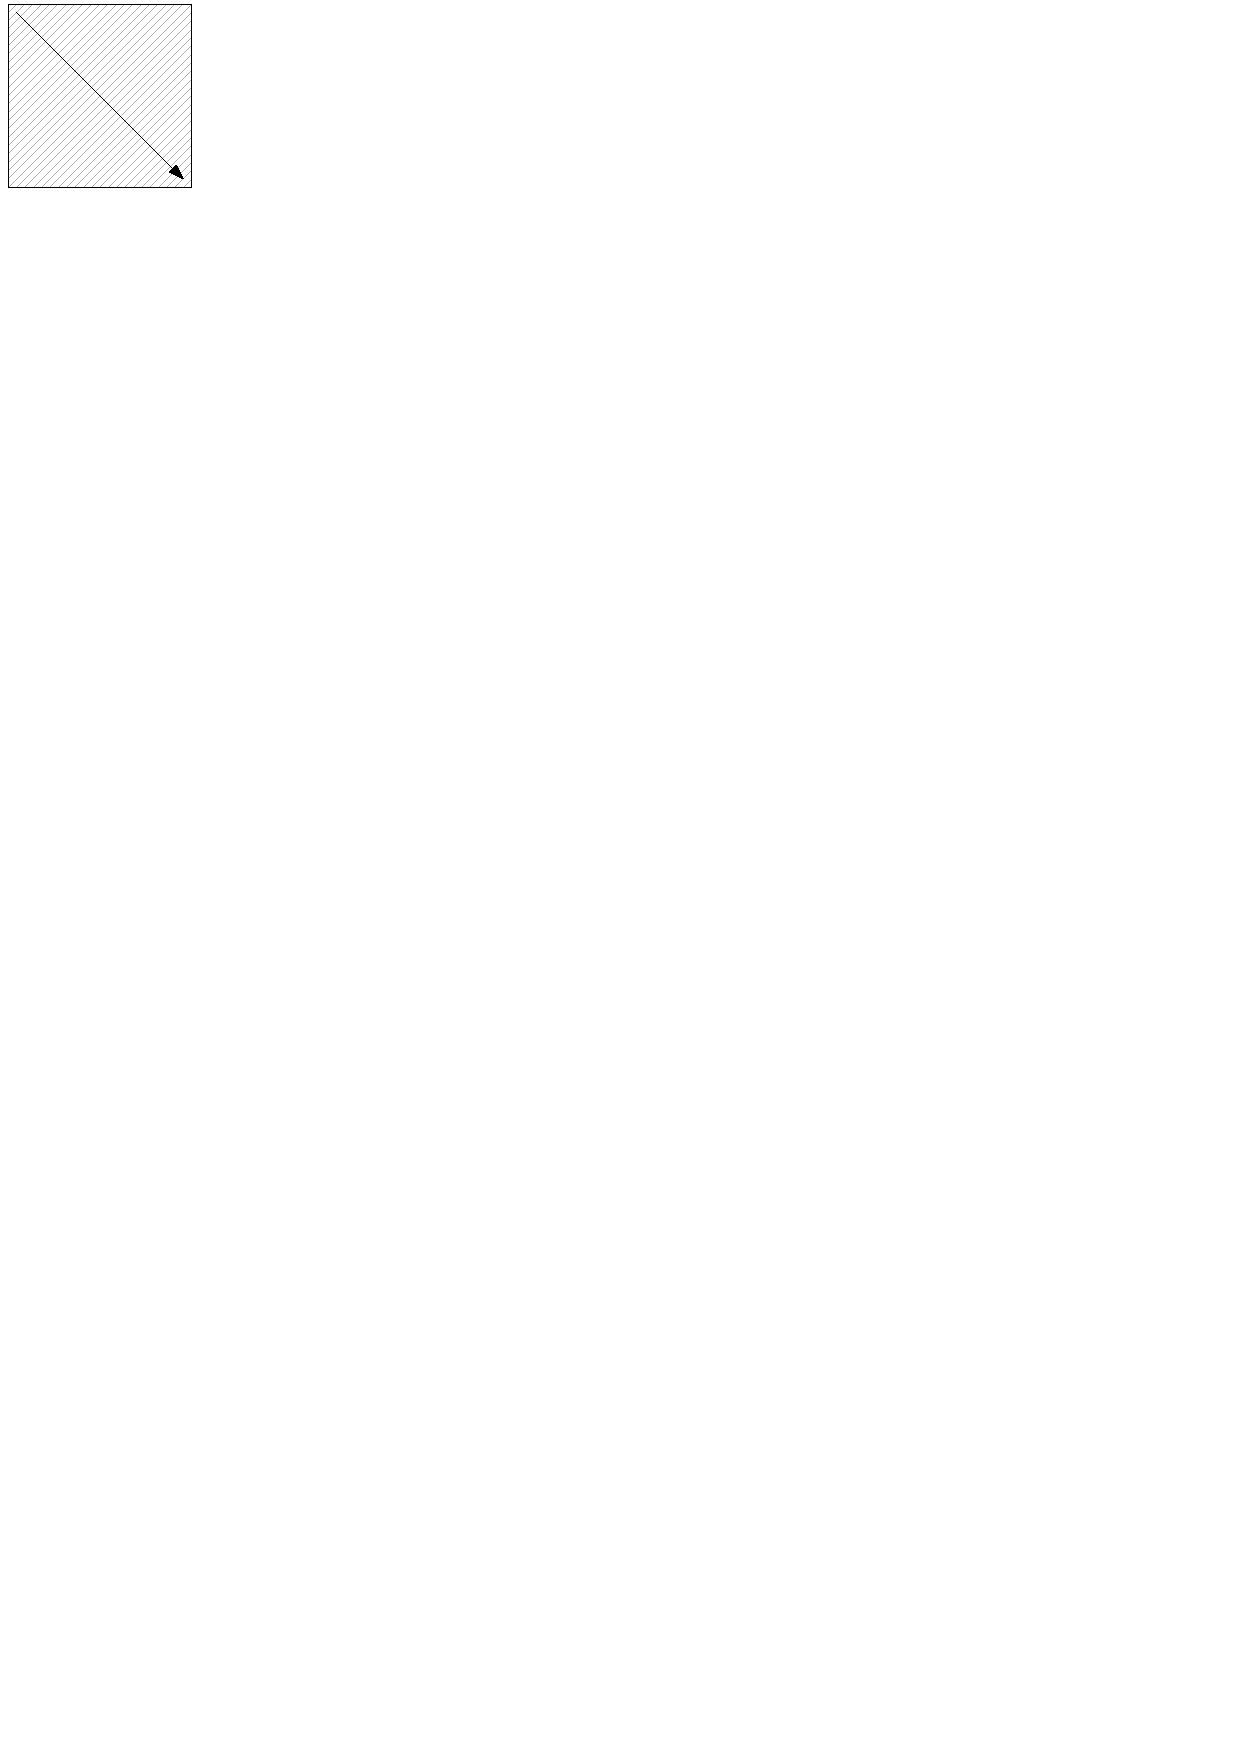
\includegraphics[scale=1.5]{../img/walkingalg1.pdf}<2>
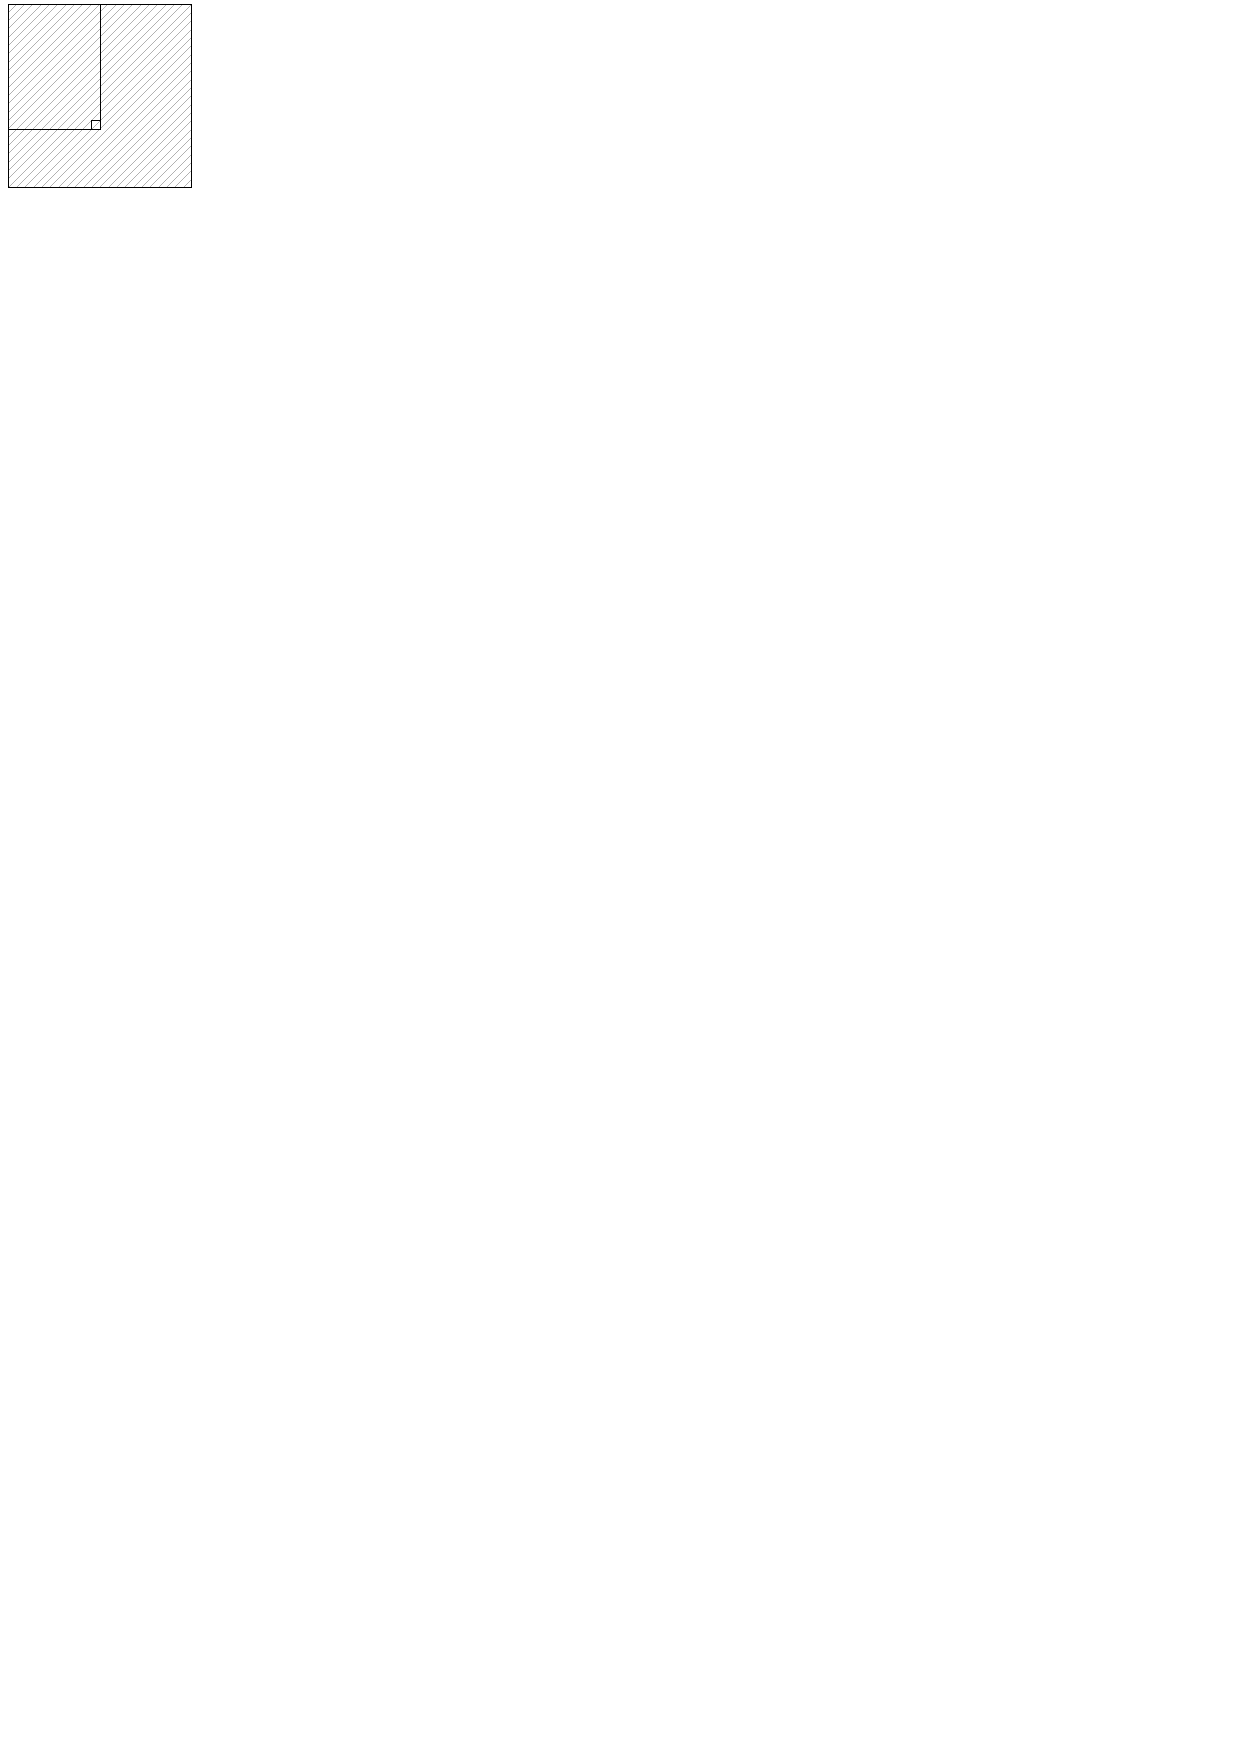
\includegraphics[scale=1.5]{../img/walkingalg2.pdf}<3>
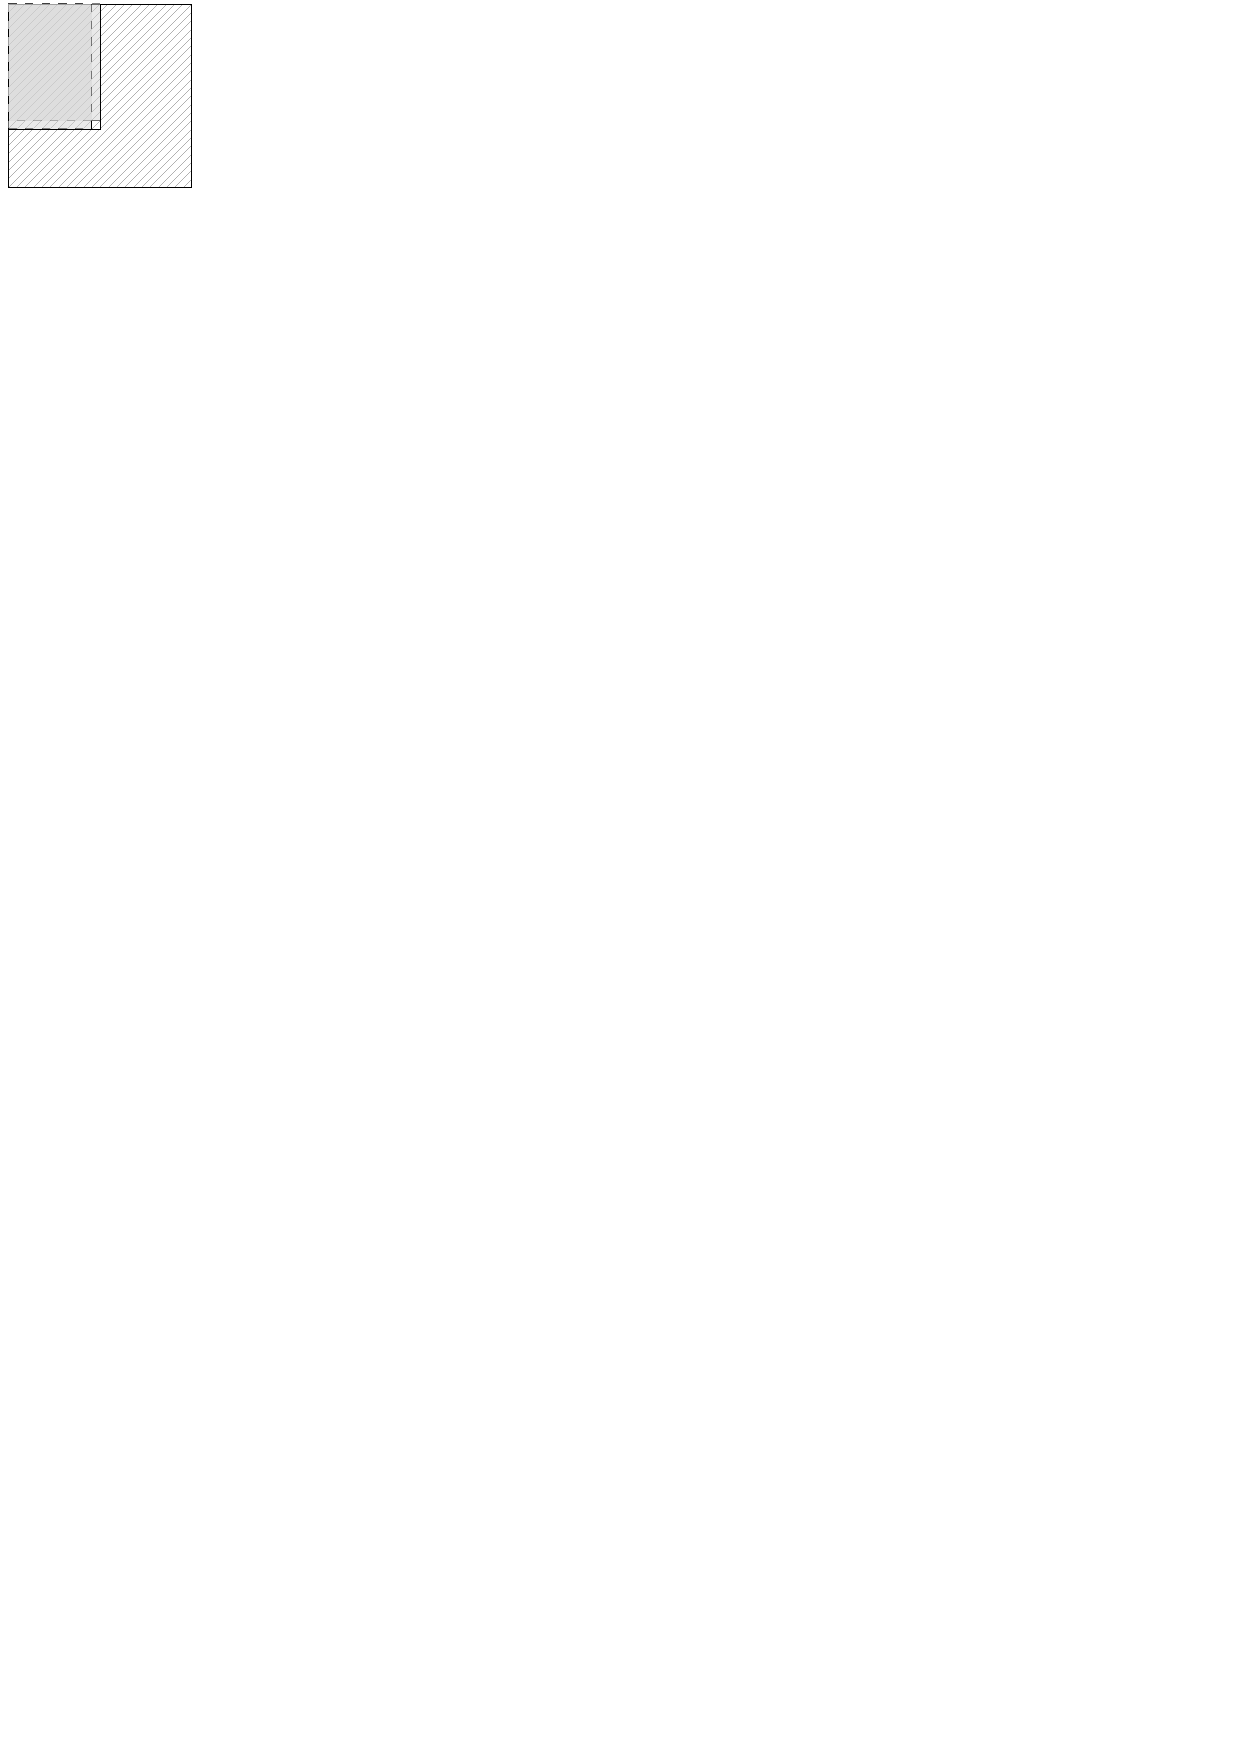
\includegraphics[scale=1.5]{../img/walkingalg3.pdf}<4>
%? c_v, c_h vynechám?
% Mejme matici, pro kterou testujeme, zda obsahuje walking_pattern. Budeme postupovat po naznačených diagonálách ve směru šipky a pro každou diagonálu a každý její prvek budeme chtít spočítat, jaká nejdelší část vzoru se vejde do podmatice určené tímto prvkem a prvním prvkem matice. Z hodnot spočítaných pro šedé matice už dokážeme v konstatním čase spočítat správnou hodnotu i pro počítaný prvek, čímž jeden test trvá lineárně dlouho s velikostí matice. Ve skutečnosti si k dosažení této složitosti potřebujeme pamatovat dvě čísla místo jednoho, ale bylo by zdlouhavé přesně zadefinovat co si pamatujeme a tento nástin by měl být dostatečný. Když během výpočtu narazíme na podmatici, do které lze namapovat i poslední prvek vzoru, pak je vzor obsažen a v opačném případě obsažen není.
% Ikdyž lineární složitost vůbec není špatná, když vezmeme v potaz že matice je velká a iterací bude hodně, je ku prospěchu nepočítat nic, co počítat nemusíme a když využijeme toho, že každá nová iterace na Markovově řetězci změní jen jeden bit, můžeme si spočítané hodnoty pamatovat i mezi iteracemi a pouze přepočítat prvky, kde se hodnota změní, což celý proces ještě uspíší.
\end{frame}

\subsection{Algoritmus pro testování obecných vzorů}
\begin{frame}
\frametitle{Algoritmus pro testování obecných vzorů}
Problém rozhodnout zda daná permutace obsahuje podpermutaci je NP-úplný. Stejný problém můžeme řešit jako otázku zda permutační matice obsahuje permutační vzor, čímž dostáváme, že rozhodování obsahování matice v~matici je NP-těžké.\\
%? Přečtu. Zase by se mohla hodit citace?
\pause
\vspace{1em}
Dva možné brute-force přístupy:
\pause
\vspace{1mm}
\begin{itemize}
\setlength\itemsep{3mm}
\item Vyzkoušet všechny možné podmatice správné velikosti.
\pause
\vspace{1mm}
\begin{itemize}
\item Implementuji jako Slow\_pattern.
\end{itemize}
\pause
\item Postupně namapovat všechny linie (řádky a~sloupce) vzoru na~všechny možné linie testované matice.
\begin{itemize}
\pause
\vspace{1mm}
\item Implementuji jako General\_pattern s~použitím mnoha výpočetních i~paměťových optimalizací.
\end{itemize}
% Na třídu General_pattern se teď podíváme trochu více.
\end{itemize}
\end{frame}

\begin{frame}
\frametitle{General\_pattern}
Při testování obsahování vzoru postupně mapujeme všechny linie (řádky a~sloupce) vzoru na~všechny možné linie testované matice.\\
\vspace{1em}
Optimalizace:
% Ve svém programu se samozřejmě snažím algoritmus mnoha způsoby optimalizovat, tady je seznam několika důležitých optimalizací.
%. Bod vždy přečtu a pak k němu něco dodám.
\begin{itemize}
\item Některá částečná mapování můžeme sloučit do~jednoho a~tím ušetřit čas~i prostor.
% To, která mapování můžeme sloučit přímo závisí na volbě pořadí linií, protože slučovat můžeme pouze ta mapování, která se liší pouze v namapování linií, které už jsou ze všech směrů omezeny.
%? Chci to popsat pořádněji?
\pause
\item Program poskytuje mnoho různých způsobů jak zvolit pořadí, ve~kterém se budou linie mapovat.
% Ač se to tak nemusí na první pohled jevit, volba pořadí je zásadní pro rychlost testování a to hlavně kvůli předchozímu bodu. Efektivita různých voleb se liší vzor od vzoru a uživatel si pořadí může zvolit.
\pause
\item Volitelně program testuje kromě toho, že jsou jedničky tam, kde být musí, také jestli je dost jedniček tam, kam se později budou mapovat dosud nenamapované linie.
\pause
% Tento popis obsahuje několikero různých heuristik, které může uživatel podle uvážení zapnout nebo vypnout a jejichž důsledkem je, že sice mapování jedné linie trvá déle, ale zase daleko rychleji poznáme, že vytvořené částečné mapování již nepůjde rozšířit na mapování celého vzoru.
\item Protože známe generující proces a již víme, že matice před změnou bitu vzor neobsahovala, víme také, že pokud ho po~změně obsahuje tak jedině proto, že právě změněný bit je součástí mapování vzoru.
% Což znovu značně zmenšuje počet částečných mapování, které v průběhu program vytvoří.
\end{itemize}
\end{frame}

%? Paralelismus? Citace?
%? Děkuji za pozornost?

\end{document}